\documentclass[twoside]{book}

% Packages required by doxygen
\usepackage{fixltx2e}
\usepackage{calc}
\usepackage{doxygen}
\usepackage[export]{adjustbox} % also loads graphicx
\usepackage{graphicx}
\usepackage[utf8]{inputenc}
\usepackage{makeidx}
\usepackage{multicol}
\usepackage{multirow}
\PassOptionsToPackage{warn}{textcomp}
\usepackage{textcomp}
\usepackage[nointegrals]{wasysym}
\usepackage[table]{xcolor}

% Font selection
\usepackage[T1]{fontenc}
\usepackage[scaled=.90]{helvet}
\usepackage{courier}
\usepackage{amssymb}
\usepackage{sectsty}
\renewcommand{\familydefault}{\sfdefault}
\allsectionsfont{%
  \fontseries{bc}\selectfont%
  \color{darkgray}%
}
\renewcommand{\DoxyLabelFont}{%
  \fontseries{bc}\selectfont%
  \color{darkgray}%
}
\newcommand{\+}{\discretionary{\mbox{\scriptsize$\hookleftarrow$}}{}{}}

% Page & text layout
\usepackage{geometry}
\geometry{%
  a4paper,%
  top=2.5cm,%
  bottom=2.5cm,%
  left=2.5cm,%
  right=2.5cm%
}
\tolerance=750
\hfuzz=15pt
\hbadness=750
\setlength{\emergencystretch}{15pt}
\setlength{\parindent}{0cm}
\setlength{\parskip}{0.2cm}
\makeatletter
\renewcommand{\paragraph}{%
  \@startsection{paragraph}{4}{0ex}{-1.0ex}{1.0ex}{%
    \normalfont\normalsize\bfseries\SS@parafont%
  }%
}
\renewcommand{\subparagraph}{%
  \@startsection{subparagraph}{5}{0ex}{-1.0ex}{1.0ex}{%
    \normalfont\normalsize\bfseries\SS@subparafont%
  }%
}
\makeatother

% Headers & footers
\usepackage{fancyhdr}
\pagestyle{fancyplain}
\fancyhead[LE]{\fancyplain{}{\bfseries\thepage}}
\fancyhead[CE]{\fancyplain{}{}}
\fancyhead[RE]{\fancyplain{}{\bfseries\leftmark}}
\fancyhead[LO]{\fancyplain{}{\bfseries\rightmark}}
\fancyhead[CO]{\fancyplain{}{}}
\fancyhead[RO]{\fancyplain{}{\bfseries\thepage}}
\fancyfoot[LE]{\fancyplain{}{}}
\fancyfoot[CE]{\fancyplain{}{}}
\fancyfoot[RE]{\fancyplain{}{\bfseries\scriptsize Generated on Tue Oct 13 2015 23\+:23\+:18 for My Project by Doxygen }}
\fancyfoot[LO]{\fancyplain{}{\bfseries\scriptsize Generated on Tue Oct 13 2015 23\+:23\+:18 for My Project by Doxygen }}
\fancyfoot[CO]{\fancyplain{}{}}
\fancyfoot[RO]{\fancyplain{}{}}
\renewcommand{\footrulewidth}{0.4pt}
\renewcommand{\chaptermark}[1]{%
  \markboth{#1}{}%
}
\renewcommand{\sectionmark}[1]{%
  \markright{\thesection\ #1}%
}

% Indices & bibliography
\usepackage{natbib}
\usepackage[titles]{tocloft}
\setcounter{tocdepth}{3}
\setcounter{secnumdepth}{5}
\makeindex

% Hyperlinks (required, but should be loaded last)
\usepackage{ifpdf}
\ifpdf
  \usepackage[pdftex,pagebackref=true]{hyperref}
\else
  \usepackage[ps2pdf,pagebackref=true]{hyperref}
\fi
\hypersetup{%
  colorlinks=true,%
  linkcolor=blue,%
  citecolor=blue,%
  unicode%
}

% Custom commands
\newcommand{\clearemptydoublepage}{%
  \newpage{\pagestyle{empty}\cleardoublepage}%
}

\usepackage{caption}
\captionsetup{labelsep=space,justification=centering,font={bf},singlelinecheck=off,skip=4pt,position=top}

%===== C O N T E N T S =====

\begin{document}

% Titlepage & ToC
\hypersetup{pageanchor=false,
             bookmarks=true,
             bookmarksnumbered=true,
             pdfencoding=unicode
            }
\pagenumbering{roman}
\begin{titlepage}
\vspace*{7cm}
\begin{center}%
{\Large My Project }\\
\vspace*{1cm}
{\large Generated by Doxygen 1.8.11}\\
\vspace*{0.5cm}
{\small Tue Oct 13 2015 23:23:18}\\
\end{center}
\end{titlepage}
\clearemptydoublepage
\tableofcontents
\clearemptydoublepage
\pagenumbering{arabic}
\hypersetup{pageanchor=true}

%--- Begin generated contents ---
\chapter{Hierarchical Index}
\section{Class Hierarchy}
This inheritance list is sorted roughly, but not completely, alphabetically\+:\begin{DoxyCompactList}
\item \contentsline{section}{Audio\+Manager}{\pageref{classAudioManager}}{}
\item \contentsline{section}{F\+FT}{\pageref{classFFT}}{}
\item \contentsline{section}{File}{\pageref{classFile}}{}
\item \contentsline{section}{File\+Manager}{\pageref{classFileManager}}{}
\item \contentsline{section}{I\+HM}{\pageref{classIHM}}{}
\item \contentsline{section}{Observer}{\pageref{classObserver}}{}
\begin{DoxyCompactList}
\item \contentsline{section}{Sound\+Wave}{\pageref{classSoundWave}}{}
\end{DoxyCompactList}
\item \contentsline{section}{Prototype$<$ T $>$}{\pageref{classPrototype}}{}
\item \contentsline{section}{Prototype$<$ File $>$}{\pageref{classPrototype}}{}
\begin{DoxyCompactList}
\item \contentsline{section}{File\+Maker}{\pageref{classFileMaker}}{}
\end{DoxyCompactList}
\item Sound\+Stream\begin{DoxyCompactList}
\item \contentsline{section}{Sound\+Stream}{\pageref{classSoundStream}}{}
\end{DoxyCompactList}
\item \contentsline{section}{Sound\+Wave\+Displayer}{\pageref{classSoundWaveDisplayer}}{}
\begin{DoxyCompactList}
\item \contentsline{section}{Line\+Displayer}{\pageref{classLineDisplayer}}{}
\end{DoxyCompactList}
\end{DoxyCompactList}

\chapter{Class Index}
\section{Class List}
Here are the classes, structs, unions and interfaces with brief descriptions\+:\begin{DoxyCompactList}
\item\contentsline{section}{\hyperlink{classAudioManager}{Audio\+Manager} \\*The \hyperlink{classAudioManager}{Audio\+Manager} handle basic operations such play, pause or stop a sound\+Stream. The audio data are stored in the buffer and are being use by \hyperlink{classSoundStream}{Sound\+Stream} to do all the hard work }{\pageref{classAudioManager}}{}
\item\contentsline{section}{\hyperlink{classFFT}{F\+FT} }{\pageref{classFFT}}{}
\item\contentsline{section}{\hyperlink{classFile}{File} }{\pageref{classFile}}{}
\item\contentsline{section}{\hyperlink{classFileMaker}{File\+Maker} }{\pageref{classFileMaker}}{}
\item\contentsline{section}{\hyperlink{classFileManager}{File\+Manager} }{\pageref{classFileManager}}{}
\item\contentsline{section}{\hyperlink{classIHM}{I\+HM} }{\pageref{classIHM}}{}
\item\contentsline{section}{\hyperlink{classLineDisplayer}{Line\+Displayer} }{\pageref{classLineDisplayer}}{}
\item\contentsline{section}{\hyperlink{classObserver}{Observer} }{\pageref{classObserver}}{}
\item\contentsline{section}{\hyperlink{classPrototype}{Prototype$<$ T $>$} }{\pageref{classPrototype}}{}
\item\contentsline{section}{\hyperlink{classSoundStream}{Sound\+Stream} }{\pageref{classSoundStream}}{}
\item\contentsline{section}{\hyperlink{classSoundWave}{Sound\+Wave} }{\pageref{classSoundWave}}{}
\item\contentsline{section}{\hyperlink{classSoundWaveDisplayer}{Sound\+Wave\+Displayer} }{\pageref{classSoundWaveDisplayer}}{}
\end{DoxyCompactList}

\chapter{Class Documentation}
\hypertarget{classaudioManager}{}\section{audio\+Manager Class Reference}
\label{classaudioManager}\index{audio\+Manager@{audio\+Manager}}
\subsection*{Public Member Functions}
\begin{DoxyCompactItemize}
\item 
{\bfseries audio\+Manager} (sf\+::\+String)\hypertarget{classaudioManager_a6beca9bae38533550aa2fd756f5ccb65}{}\label{classaudioManager_a6beca9bae38533550aa2fd756f5ccb65}

\item 
bool {\bfseries load\+Music} (sf\+::\+String=\char`\"{}\char`\"{})\hypertarget{classaudioManager_ada6c910430c0c1e7467ad8c6641010f7}{}\label{classaudioManager_ada6c910430c0c1e7467ad8c6641010f7}

\item 
void {\bfseries play} ()\hypertarget{classaudioManager_aa81e9bae4581eb3a4e745635f7245927}{}\label{classaudioManager_aa81e9bae4581eb3a4e745635f7245927}

\item 
void {\bfseries pause} ()\hypertarget{classaudioManager_a915f6accefbcd9ee687b9aa913b5be5f}{}\label{classaudioManager_a915f6accefbcd9ee687b9aa913b5be5f}

\item 
void {\bfseries stop} ()\hypertarget{classaudioManager_a24d4746810b66c3c5db3d041ce37ab36}{}\label{classaudioManager_a24d4746810b66c3c5db3d041ce37ab36}

\item 
void {\bfseries seek} (sf\+::\+Time)\hypertarget{classaudioManager_ae25f98a4737421d17abb94162495faf0}{}\label{classaudioManager_ae25f98a4737421d17abb94162495faf0}

\end{DoxyCompactItemize}


The documentation for this class was generated from the following files\+:\begin{DoxyCompactItemize}
\item 
header/audio\+Manager.\+h\item 
src/audio\+Manager.\+cpp\end{DoxyCompactItemize}

\hypertarget{classFFT}{}\section{F\+FT Class Reference}
\label{classFFT}\index{F\+FT@{F\+FT}}
\subsection*{Public Member Functions}
\begin{DoxyCompactItemize}
\item 
void {\bfseries power\+Spectrum} (int start, int half, float $\ast$data, int window\+Size, float $\ast$magnitude, float $\ast$phase, float $\ast$power, float $\ast$avg\+\_\+power)\hypertarget{classFFT_ad038ab187e20c4f628545f51b8822a1b}{}\label{classFFT_ad038ab187e20c4f628545f51b8822a1b}

\item 
void {\bfseries inverse\+Power\+Spectrum} (int start, int half, int window\+Size, float $\ast$final\+Out, float $\ast$magnitude, float $\ast$phase)\hypertarget{classFFT_a2f17d2309d72e26032d8909fa7bfd016}{}\label{classFFT_a2f17d2309d72e26032d8909fa7bfd016}

\end{DoxyCompactItemize}


The documentation for this class was generated from the following files\+:\begin{DoxyCompactItemize}
\item 
header/F\+F\+T.\+h\item 
src/F\+F\+T.\+cpp\end{DoxyCompactItemize}

\hypertarget{classIHM}{}\section{I\+HM Class Reference}
\label{classIHM}\index{I\+HM@{I\+HM}}
\subsection*{Public Member Functions}
\begin{DoxyCompactItemize}
\item 
\hyperlink{classIHM_aade5baff871034cb667f43930620c121}{I\+HM} ()\hypertarget{classIHM_aade5baff871034cb667f43930620c121}{}\label{classIHM_aade5baff871034cb667f43930620c121}

\begin{DoxyCompactList}\small\item\em ctor \end{DoxyCompactList}\item 
\hyperlink{classIHM_af220622a4304f5a9ed1da28abb7da14d}{$\sim$\+I\+HM} ()
\item 
void \hyperlink{classIHM_a82bd5aa63da77245548a70b73bfd2bb7}{Run} ()\hypertarget{classIHM_a82bd5aa63da77245548a70b73bfd2bb7}{}\label{classIHM_a82bd5aa63da77245548a70b73bfd2bb7}

\begin{DoxyCompactList}\small\item\em starting point of the G\+UI \end{DoxyCompactList}\end{DoxyCompactItemize}


\subsection{Constructor \& Destructor Documentation}
\index{I\+HM@{I\+HM}!````~I\+HM@{$\sim$\+I\+HM}}
\index{````~I\+HM@{$\sim$\+I\+HM}!I\+HM@{I\+HM}}
\subsubsection[{$\sim$\+I\+H\+M()}]{\setlength{\rightskip}{0pt plus 5cm}I\+H\+M\+::$\sim$\+I\+HM (
\begin{DoxyParamCaption}
{}
\end{DoxyParamCaption}
)}\hypertarget{classIHM_af220622a4304f5a9ed1da28abb7da14d}{}\label{classIHM_af220622a4304f5a9ed1da28abb7da14d}
dtor 

The documentation for this class was generated from the following files\+:\begin{DoxyCompactItemize}
\item 
header/I\+H\+M.\+h\item 
src/I\+H\+M.\+cpp\end{DoxyCompactItemize}

\hypertarget{classSoundStream}{}\section{Sound\+Stream Class Reference}
\label{classSoundStream}\index{Sound\+Stream@{Sound\+Stream}}
Inheritance diagram for Sound\+Stream\+:\begin{figure}[H]
\begin{center}
\leavevmode
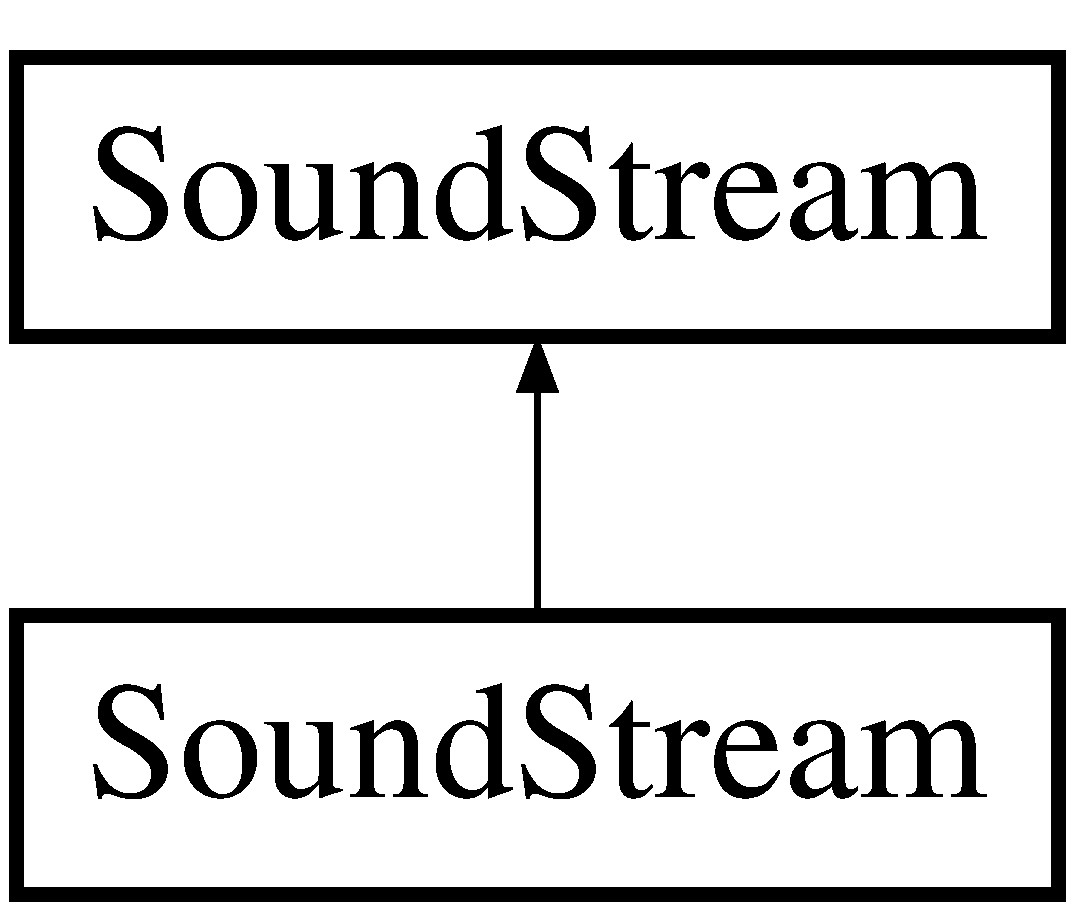
\includegraphics[height=2.000000cm]{classSoundStream}
\end{center}
\end{figure}
\subsection*{Public Member Functions}
\begin{DoxyCompactItemize}
\item 
void \hyperlink{classSoundStream_a65c3f112bdc3373c231ddcd0767fd031}{load} (const sf\+::\+Sound\+Buffer \&)
\item 
void \hyperlink{classSoundStream_ae7d7a1c32e012792a9bba1df6e121e83}{seek} (sf\+::\+Time)\hypertarget{classSoundStream_ae7d7a1c32e012792a9bba1df6e121e83}{}\label{classSoundStream_ae7d7a1c32e012792a9bba1df6e121e83}

\begin{DoxyCompactList}\small\item\em load \end{DoxyCompactList}\end{DoxyCompactItemize}


\subsection{Member Function Documentation}
\index{Sound\+Stream@{Sound\+Stream}!load@{load}}
\index{load@{load}!Sound\+Stream@{Sound\+Stream}}
\subsubsection[{load(const sf\+::\+Sound\+Buffer \&)}]{\setlength{\rightskip}{0pt plus 5cm}void Sound\+Stream\+::load (
\begin{DoxyParamCaption}
\item[{const sf\+::\+Sound\+Buffer \&}]{buffer}
\end{DoxyParamCaption}
)}\hypertarget{classSoundStream_a65c3f112bdc3373c231ddcd0767fd031}{}\label{classSoundStream_a65c3f112bdc3373c231ddcd0767fd031}
\hyperlink{classSoundStream}{Sound\+Stream} \+: Public 

The documentation for this class was generated from the following files\+:\begin{DoxyCompactItemize}
\item 
header/Sound\+Stream.\+h\item 
src/Sound\+Stream.\+cpp\end{DoxyCompactItemize}

\hypertarget{classSoundWave}{}\section{Sound\+Wave Class Reference}
\label{classSoundWave}\index{Sound\+Wave@{Sound\+Wave}}
Inheritance diagram for Sound\+Wave\+:\begin{figure}[H]
\begin{center}
\leavevmode
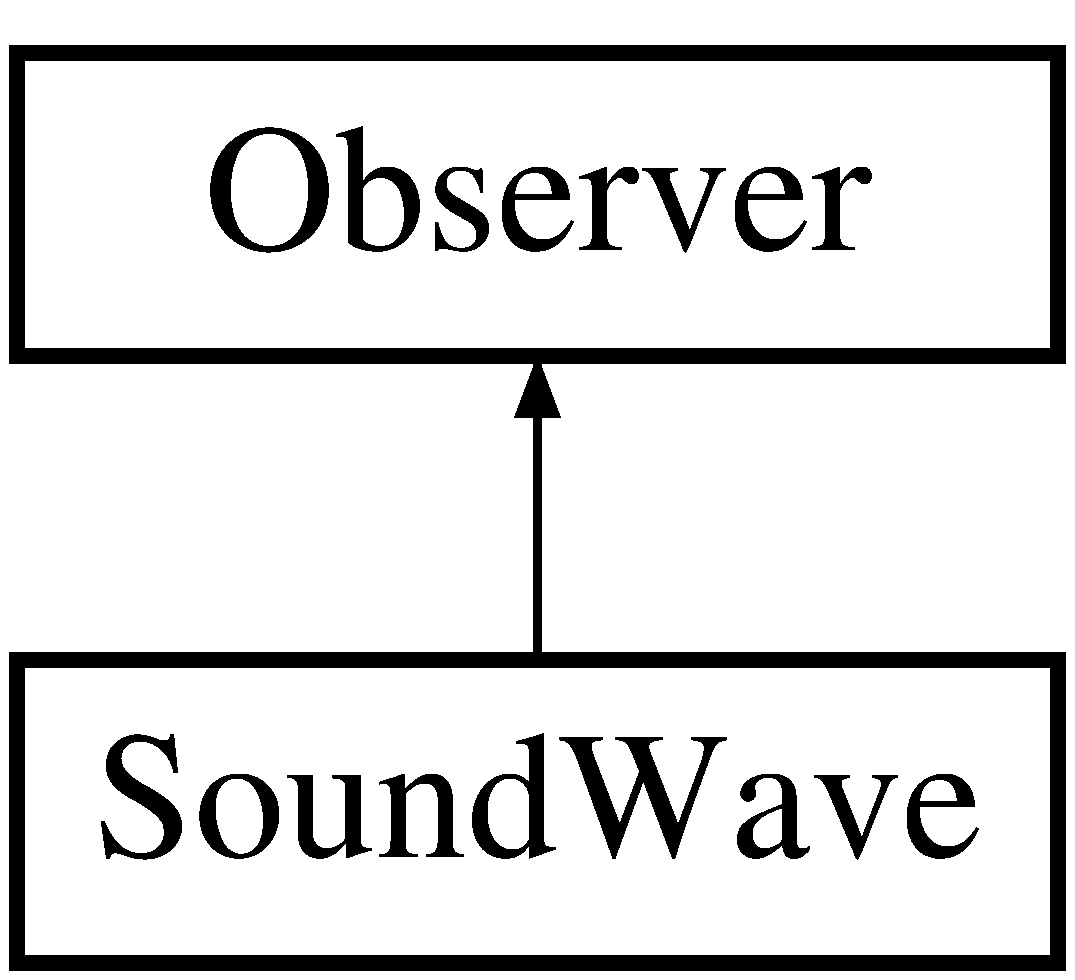
\includegraphics[height=2.000000cm]{classSoundWave}
\end{center}
\end{figure}
\subsection*{Public Member Functions}
\begin{DoxyCompactItemize}
\item 
\hyperlink{classSoundWave_afbbc5fd5ede5570ff4ba4b41e8df7c5b}{Sound\+Wave} ()
\begin{DoxyCompactList}\small\item\em default ctor \end{DoxyCompactList}\item 
virtual \hyperlink{classSoundWave_aea2c03780b6e04f41319b7f4a09bbec1}{$\sim$\+Sound\+Wave} ()
\item 
int \hyperlink{classSoundWave_a44a2aaac4bb3690a0f60dac48d37adc3}{get\+Buffer\+Size} ()
\begin{DoxyCompactList}\small\item\em return the Buffer\+Size \end{DoxyCompactList}\item 
void \hyperlink{classSoundWave_ab8dfd69deeffc8f7f9fccd221708a750}{init} ()\hypertarget{classSoundWave_ab8dfd69deeffc8f7f9fccd221708a750}{}\label{classSoundWave_ab8dfd69deeffc8f7f9fccd221708a750}

\begin{DoxyCompactList}\small\item\em init the soundwave data \end{DoxyCompactList}\item 
float $\ast$ \hyperlink{classSoundWave_a0ef0523616554bbf5ca3a7c5bcccf347}{get\+Magnitude} ()\hypertarget{classSoundWave_a0ef0523616554bbf5ca3a7c5bcccf347}{}\label{classSoundWave_a0ef0523616554bbf5ca3a7c5bcccf347}

\begin{DoxyCompactList}\small\item\em return the magnitude array \end{DoxyCompactList}\item 
float $\ast$ \hyperlink{classSoundWave_a53e58f2e72dba0a8c6166faa9831559a}{get\+Phase} ()\hypertarget{classSoundWave_a53e58f2e72dba0a8c6166faa9831559a}{}\label{classSoundWave_a53e58f2e72dba0a8c6166faa9831559a}

\begin{DoxyCompactList}\small\item\em return the phase array \end{DoxyCompactList}\item 
float $\ast$ \hyperlink{classSoundWave_af7a8ad9411b800f5c40171d0cb7f5655}{get\+Power} ()\hypertarget{classSoundWave_af7a8ad9411b800f5c40171d0cb7f5655}{}\label{classSoundWave_af7a8ad9411b800f5c40171d0cb7f5655}

\begin{DoxyCompactList}\small\item\em return the power array \end{DoxyCompactList}\item 
float \hyperlink{classSoundWave_ae9ee9576dc02cc46bd73c38b59d58cb2}{get\+Avg\+Power} ()\hypertarget{classSoundWave_ae9ee9576dc02cc46bd73c38b59d58cb2}{}\label{classSoundWave_ae9ee9576dc02cc46bd73c38b59d58cb2}

\begin{DoxyCompactList}\small\item\em return the avg\+Power \end{DoxyCompactList}\end{DoxyCompactItemize}


\subsection{Constructor \& Destructor Documentation}
\index{Sound\+Wave@{Sound\+Wave}!Sound\+Wave@{Sound\+Wave}}
\index{Sound\+Wave@{Sound\+Wave}!Sound\+Wave@{Sound\+Wave}}
\subsubsection[{Sound\+Wave()}]{\setlength{\rightskip}{0pt plus 5cm}Sound\+Wave\+::\+Sound\+Wave (
\begin{DoxyParamCaption}
{}
\end{DoxyParamCaption}
)}\hypertarget{classSoundWave_afbbc5fd5ede5570ff4ba4b41e8df7c5b}{}\label{classSoundWave_afbbc5fd5ede5570ff4ba4b41e8df7c5b}


default ctor 

\begin{DoxySeeAlso}{See also}
\hyperlink{classSoundWave_afbbc5fd5ede5570ff4ba4b41e8df7c5b}{Sound\+Wave()}default ctor 
\end{DoxySeeAlso}
\index{Sound\+Wave@{Sound\+Wave}!````~Sound\+Wave@{$\sim$\+Sound\+Wave}}
\index{````~Sound\+Wave@{$\sim$\+Sound\+Wave}!Sound\+Wave@{Sound\+Wave}}
\subsubsection[{$\sim$\+Sound\+Wave()}]{\setlength{\rightskip}{0pt plus 5cm}Sound\+Wave\+::$\sim$\+Sound\+Wave (
\begin{DoxyParamCaption}
{}
\end{DoxyParamCaption}
)\hspace{0.3cm}{\ttfamily [virtual]}}\hypertarget{classSoundWave_aea2c03780b6e04f41319b7f4a09bbec1}{}\label{classSoundWave_aea2c03780b6e04f41319b7f4a09bbec1}
dtor 

\subsection{Member Function Documentation}
\index{Sound\+Wave@{Sound\+Wave}!get\+Buffer\+Size@{get\+Buffer\+Size}}
\index{get\+Buffer\+Size@{get\+Buffer\+Size}!Sound\+Wave@{Sound\+Wave}}
\subsubsection[{get\+Buffer\+Size()}]{\setlength{\rightskip}{0pt plus 5cm}int Sound\+Wave\+::get\+Buffer\+Size (
\begin{DoxyParamCaption}
{}
\end{DoxyParamCaption}
)}\hypertarget{classSoundWave_a44a2aaac4bb3690a0f60dac48d37adc3}{}\label{classSoundWave_a44a2aaac4bb3690a0f60dac48d37adc3}


return the Buffer\+Size 

\begin{DoxySeeAlso}{See also}
B\+U\+F\+F\+E\+R\+\_\+\+S\+I\+ZE 
\end{DoxySeeAlso}
\begin{DoxyReturn}{Returns}
buffer size 
\end{DoxyReturn}


The documentation for this class was generated from the following files\+:\begin{DoxyCompactItemize}
\item 
header/Sound\+Wave.\+h\item 
src/Sound\+Wave.\+cpp\end{DoxyCompactItemize}

%--- End generated contents ---

% Index
\backmatter
\newpage
\phantomsection
\clearemptydoublepage
\addcontentsline{toc}{chapter}{Index}
\printindex

\end{document}
